\subsubsection{Feature selection - Dataset connection and variable filter}\label{feature-selection}

The original dataset \cite{divvy} is divided into years and each year into multiple parts. Therefore, the first task of all has been the union of each of these parts into a single file. The file format offered by Divvy is in a \acrshort{csv} as usual, and therefore the pandas \small{\verb|read_csv|} \normalsize  function that converts a \acrshort{csv} to a \small{\verb|DataFrame|} \normalsize  has been mainly used. On the other hand, each part had its own nomenclature of columns so it has been necessary to create a single nomenclature to work with a single file and therefore some columns have been renamed. Once the renaming of columns has been carried out, the \small{\verb|DataFrame|} \normalsize will be attached to another one that will contain all the data and which will be used for the following steps.


\begin{displayquote}
"A \small{\verb|DataFrame|} \normalsize  is a 2-dimensional labeled data structure with columns of potentially different types. You can think of it as a spreadsheet or a \acrshort{sql} table. It is generally the most commonly used object in the pandas library". \cite{pandas}
\end{displayquote}


An example of \small{\verb|DataFrame|} \normalsize  that has been seen before could be table 2. To be able to initialise a \small{\verb|DataFrame|} \normalsize  it can be done from a Python dictionary, where each key is the \small{\verb|string|} \normalsize  that identifies the column and each value is a vector with the same amount of values that rows want to have. Another way to initialise a \small{\verb|DataFrame|} \normalsize  is by using functions like \small{\verb|read_csv()|} \normalsize , \small{\verb|read_h5()|} \normalsize  or \small{\verb|read_pickle()|} \normalsize .
\newline

The code used is something like the following: 

\begin{minted}[fontsize=\footnotesize]{python}
import pandas as pd

# Path to the csv files
csv_filenames = ["trips-2014-Q1", "trips-2014-Q2-Q3", 
                 "trips-2014-Q4", "trips-2015-Q1-Q2",
                 # ...
                 "trips-2019-Q3-Q4"]
csv_paths = [f"/path/to/{file}.csv" for file in csv_filenames]

# This will be the final DataFrame
df = pd.DataFrame()

# For every CSV do
for path in csv_paths:
    
    # CSV to DataFrame
    df_temp = pd.read_csv(path)
    
    # Parse date as datetime which is always first column
    df_temp[cols[0]] = pd.to_datetime(
        df_temp[cols[0]], 
        format='%Y-%m-%d %H:%M:%S',
        infer_datetime_format=True)
    
    # Rename the columns depending on their
    # current names with a external function
    df_temp = rename_columns(df_temp)
    
    # Merge the DataFrames
    df = pd.concat([df, df_temp], join='outer')

# ...
\end{minted}


Once the \small{\verb|df|} \normalsize  variable is obtained, which collects all the trips, a filtering of the columns is necessary. At this point, the \small{\verb|DataFrame|} \normalsize  contains $12$ values associated with each trip. 

\begin{minted}[fontsize=\footnotesize]{python}
df.columns

'''
Index(['trip_id', 'start_time', 'end_time', 'bikeid', 
       'tripduration', 'from_station_id', 
       'from_station_name', 'to_station_id',
       'to_station_name', 'usertype', 'gender',
       'birthyear'],
      dtype='object')
'''
\end{minted}

Only two are selected from this \small{\verb|DataFrame|} \normalsize :

\begin{itemize}
    \item \small{\verb|start_time|} \normalsize : This data is necessary because we want to predict the use of bicycles based on temporary information. This value, given in seconds using the format "Unix Time" \cite{unix_time} allows to identify at what date and time the trip started among other data. Thanks to this, different patterns can be identified, as these vary during the time of year. There are not the same patterns during the winter as during the summer, or even, it is not the same at 2 in the morning as at 2 in the afternoon.
    
    \item \small{\verb|from_station_id|} \normalsize : The models to be built will predict the number of trips that will start at each station in Chicago independently. This value will therefore be used to calculate the number of trips started at an interval at each station. A similar task would have been to predict the number of trips that end at each station for an interval and thus control the flow of bicycles through the station network. If that had been the case, it would have been necessary to make use of \small{\verb|to_station_id|} \normalsize  and repeat the same process explained from this point on.
\end{itemize}

The other attributes are also useful for other types of problems such as predicting the most likely destination based on the station where the journey starts, or obtaining which connections are the most travelled. However, it is outside the objectives that have been set for this work so only the previously mentioned columns will be used.
\newline
 
 
The resulting dataset is therefore the same as the original dataset but with only the \small{\verb|start_time|} \normalsize  and \small{\verb|from_station_id|} \normalsize  columns. In the code this is easy to implement by adding only the following line:

\begin{minted}[fontsize=\footnotesize]{python}
# ...
    
# Filter the columns that we need
cols = ["start_time", "from_station_id"]
df = df[cols]

# Save the DataFrame in a CSV
df.to_csv("trips.csv", index=False)
\end{minted}

More columns could have been used to help predict other than those already filtered, however, due to lack of time and because the results obtained were already quite good, it has not been necessary to add them. This is discussed further in section \ref{future_work} below.
\newline

Graphically this module does the following:
\begin{figure}[H]
    \centering
    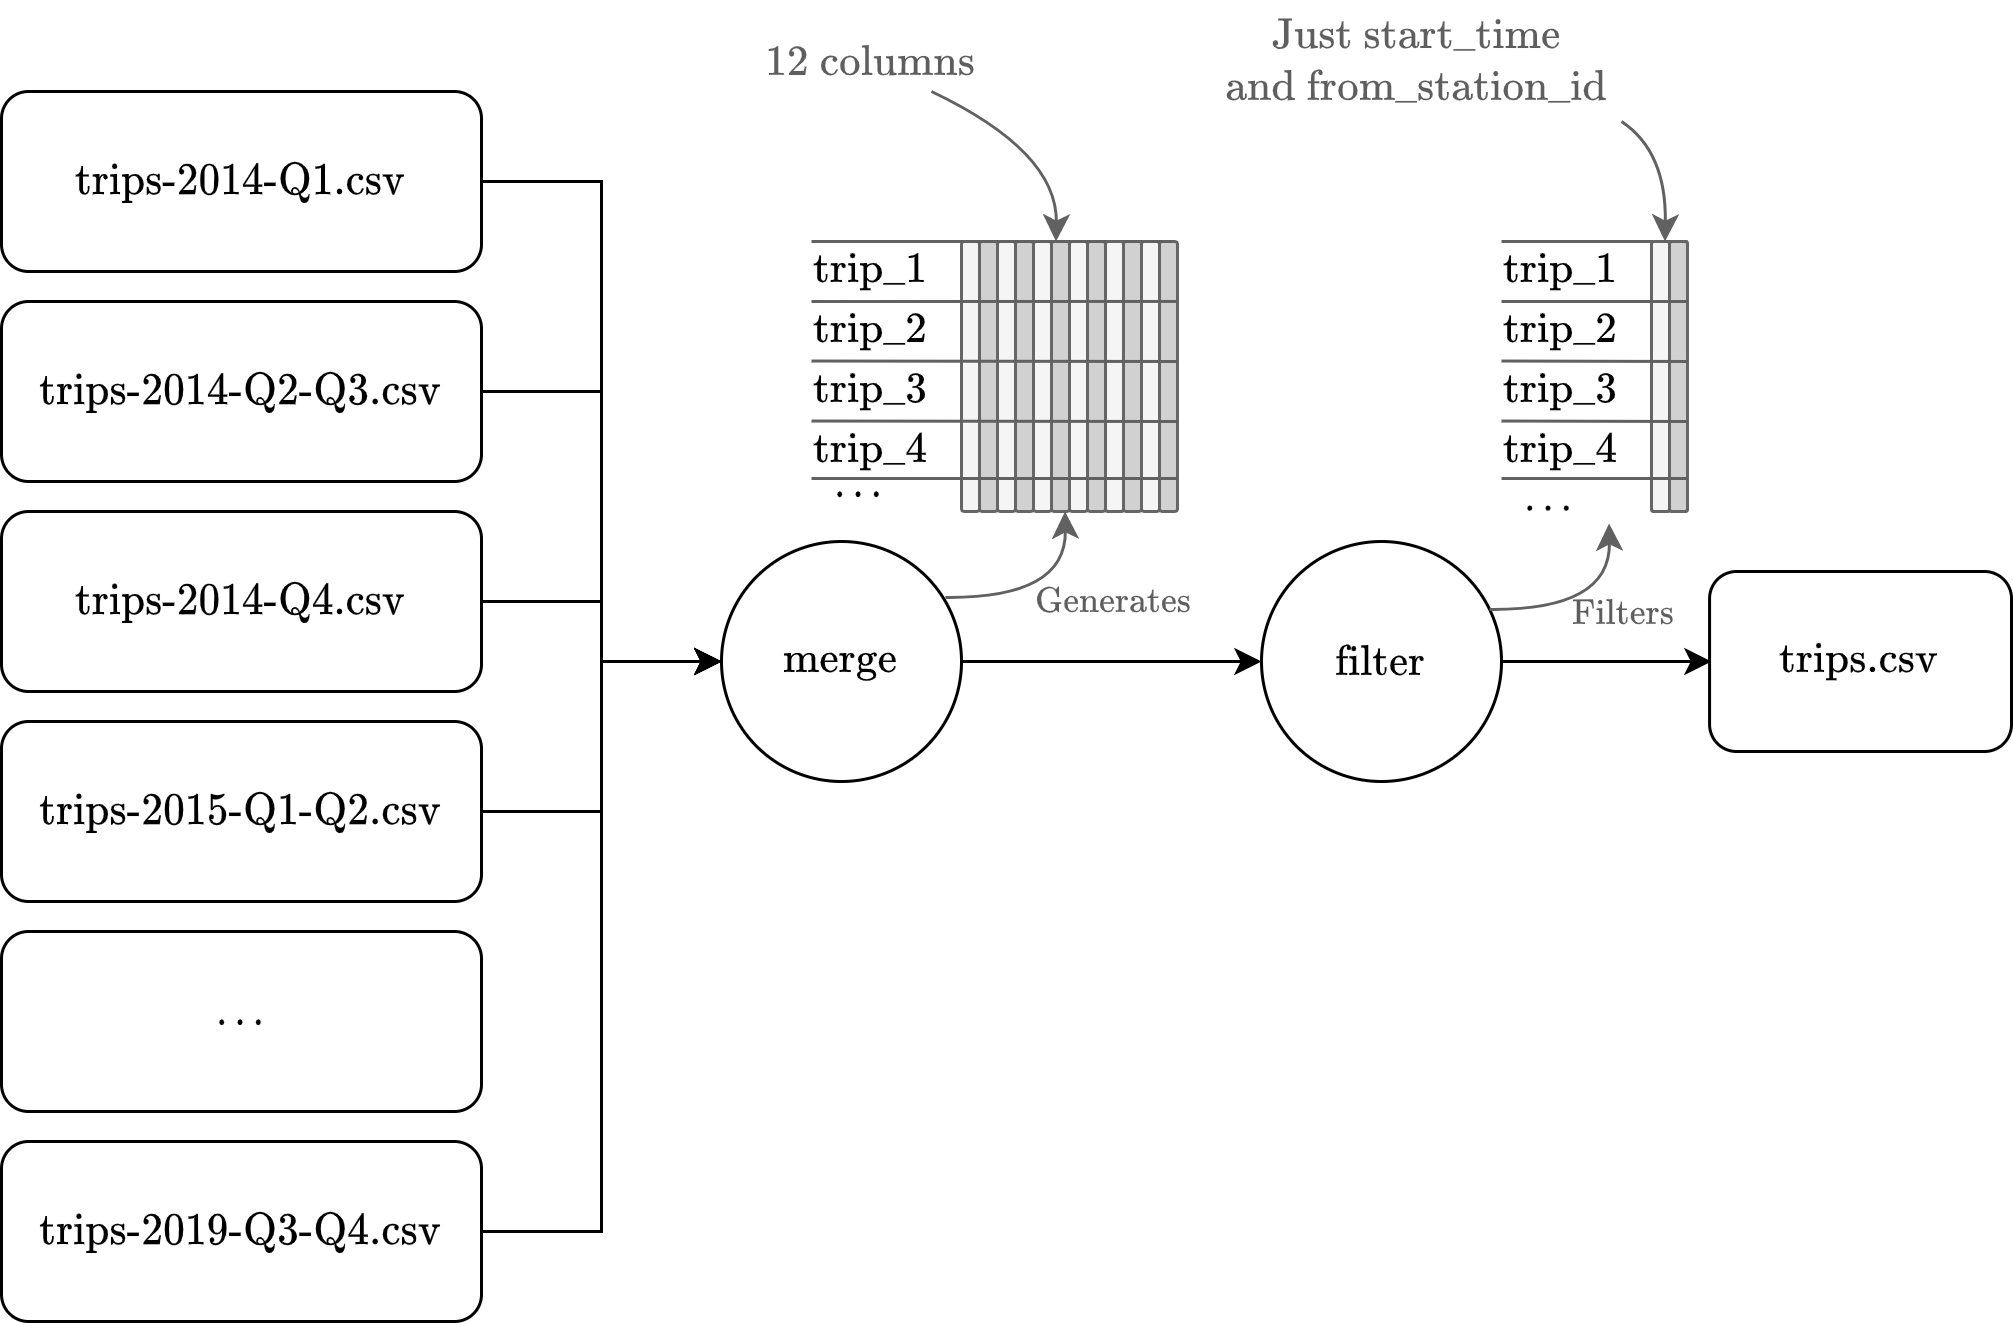
\includegraphics[width=12cm]{images/solution/modules/feature-selection.png}
    \caption{Structure of the feature-selection module}
\end{figure}